\section{Architectures}
In questa prima sezione verranno esaminate le varie architetture che sono state progettate e sintetizzate per il moltiplicatore floating point

\subsection{Classic Architecture}
Il punto di partenza della progettazione è stato il floating point pipelined multiplier a 32 bit, del quale è stato fornito il codice vhdl.
Lo schema di massima è mostrato in \autoref{fig:mult_struct}, è suddiviso in 4 stage principali:
\begin{itemize}
\item Stage 1: Viene effettuato l'unpacking dei due numeri floating point in ingresso.
\item Stage 2: Viene effettuata la moltiplicazione dei significands, trattati come numeri interi.
\item Stage 3: Viene effettuato il rounding dei significands.
\item Stage 4: Viene effettuato il calcolo dell'esponente e infine viene trasformato nuovamente il numero in floating point tramite il blocco di packing.
\end{itemize}

\begin{figure}[h]
	\center
	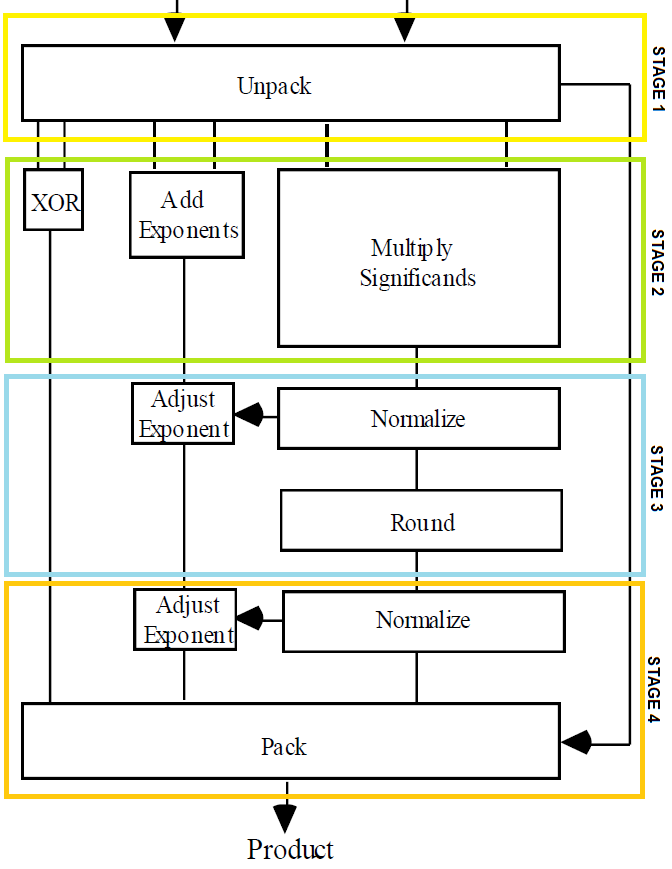
\includegraphics[width=0.6\textwidth]{mult_structure.png}
	\caption{Structure of the floating point multiplier}
	\label{fig:mult_struct}
\end{figure}

\noindent Studiando il codice VHDL si nota inolte che tra uno stadio e l'altro sono sempre presenti dei registri che campionano il segnale sul fronte di salita del clock. Per questo si può affermare che gli stage funzionali corrispondono agli stage di pipeline.
\todo{E'GIUSTO?}
Un'altra osservazione che è possibile fare su questa architettura standard è che nel secondo stage, il tipo di moltiplicatore utilizzato per moltiplicare i significands non è specificato infatti è presente un process nel quale viene fatta l'operazione con il simbolo "*" che lascia completa libertà al sintetizzatore nella scelta dell'implementazione hardware.

\subsubsection{Testbench}

Prima di partire con le varie modifiche dell'hardware è stato simulato tramite Modelsim il corretto funzionamento del circuito fornito. E' stato creato un testbench in verilog con i blocchi relativi alla generazione degli input, al DUT e al salvataggio degli output.
Come file di ingresso è stato utilizzato quello fornito sia per l'ingresso $A$ sia per $B$ di conseguenza il moltiplicatore effettuava il quadrato del numero in questione. I numeri erano rappresentati su 8 bit esadecimali quindi prima di fornirli al DUT è stata effettuata la conversione in binario.
Infine, confrontando i risultati ottenuti con quelli forniti come esempio, è stato possibile confermare il funzionamento del circuito. Inoltre studiando il timing generato da Modelsim si nota come effettivamente la latenza del circuito sia quella ipotizzata.
\\
\todo{GIUSTO?}
Successivamente è stato modificato il codice VHDL in modo da aggiungere ai segnali di ingresso dei registri; questa correzione serve a svincolare il timing degli ingressi, con eventuali glitch, dal timing interno del circuito.
A fronte di questa modifica è stato effettuato un secondo testbench, funzionalmente uguale al precedente, che ha mostrato anche in questo caso che il circuito sotto esame funzionasse correttamente.

\subsection{Stage 2 CSA PPARCH}
\todo{spiegare cosa da classic e il comando di sintesi utilizzato}

\subsection{Fine grain pipelining}
\todo{compile and compile ultra spiegare}

\subsection{MBE}
\todo{spigare struttura MBE , Dadda}
\subsubsection{Testbench}
